\documentclass[12pt, block=fill]{beamer} 
\usepackage[sfdefault]{FiraSans}
\usepackage{FiraMono}
\usepackage[T1]{fontenc}
\usepackage{xcolor}

\usepackage{pgfpages}
\setbeameroption{hide notes} % Only slides
% \setbeameroption{show only notes} % Only notes
  % \setbeameroption{show notes on second screen=right} % Both

\definecolor{burntOrange}{rgb}{.8, .5, .1}
\definecolor{textgray}{rgb}{.8,.8,.8}

\usetheme[titleformat frame = smallcaps]{metropolis}

\metroset{block=fill}

\newcommand{\E}{\text{E}}
\newcommand{\V}{\text{V}}
\newcommand{\cov}{\text{cov}}

\title{Week 6}
\subtitle{Hypothesis Testing}

\author{Paul Laskowski and D. Alex Hughes}
\institute{UC Berkeley, School of Information}

\begin{document}

\begin{frame}
  \maketitle
\end{frame}

\section{Historical Development of Frequentist Statistics}
\begin{frame}
  \frametitle{Introduction}
  \begin{itemize}
    \item Hypothesis, H, is a model for how the world might work
    \item In practice, evidence is rarely conclusive
    \item We want $Pr(H|D)$, or the probability of the event that our hypothesis is true
  \end{itemize}
\end{frame}


\begin{frame}
  \frametitle{The Dilemma}
     Whether our hypothesis is true is something we can never know 
  \begin{itemize}
    \item The world is not a perfectly controlled lab
    \item Evidence collected contains information but does not begin to identify a unique model out of all the possible models
    \item We do not know how to weight all the possibilities out there
 \end{itemize}
\end{frame}

\begin{frame}
  \frametitle{Example 1}
  \begin{exampleblock}{You flip a coin once and it lands on heads}
    What is the probability that it is a double-headed coin?
  \end{exampleblock}
  \textit{Is there enough information to answer this?}
  \begin{itemize}
    \item How did the coin get there?
    \item The context is missing:
    \begin{itemize}
        \item How do we choose between the different models?
        \item How do we weight all the alternatives?
    \end{itemize}  
    \item Even with more information, you can never know the context completely
  \end{itemize}
\end{frame}

\begin{frame}
  \frametitle{Example 2}
  \begin{exampleblock}{Isaac Newton}
    Both motions are consistent with a gravitation attraction that is proportional to the square of the distance between the objects
  \end{exampleblock}
    \begin{itemize}
        \item What is the probability that Newton's theory of gravity is correct?
        \item \textbf{Problem:} Newton's second theory seemed to work up to the precision of 17th-century instruments
        \item Only later were instruments developed that were precise enough to show Newton's laws were incorrect
    \end{itemize}
    
\end{frame}

\begin{frame}
  \frametitle{Example 2 (cont.)}

  \begin{itemize}

    \item How could Newton decide how probable his model was compared to general relativity (not imagined yet)?
    \item If he could have imagined another theory, would we be equipped to compare two very different ideas?
     \item We could never write down the infinite number of models consistent with observations of the planet in order to assign each a probability
    \item It may not even make sense to assign a probability to Newton's gravity (eg. true state of world or not)
  \end{itemize}
\end{frame}

\begin{frame}
  \frametitle{Example 3}
  You discover three specimens of a new species of squid that measure 3.2, 3.3, and 4.0 feet long
  \begin{itemize}
  \item What is the probability that the average length amount the entire species is 3.5 feet?
  
    \begin{itemize}
      \item Probability zero for a single number (point estimate)
  probability that the average length is between 3 and 4 feet?
        \item Positive number for length
        \item No new numbers that have not been imagined
        \item A better grasp of the possibilities
    \end{itemize}
  \end{itemize}
\end{frame}

\begin{frame}

\frametitle{Example 3 (cont.)}
  
    \begin{itemize}
        \item However, we don't know how representative the specimens are
        \begin{itemize}
            \item We still don't know all the relevant information
            \item Examples: deep water pressure, amount of light
        \end{itemize}
  \end{itemize}    
  \textbf{We cannot deduce the probability of our model because we do not know enough about the structure of the world} 
\end{frame}

\begin{frame}
  \frametitle{Two Branches of Statistics }
  \centering
  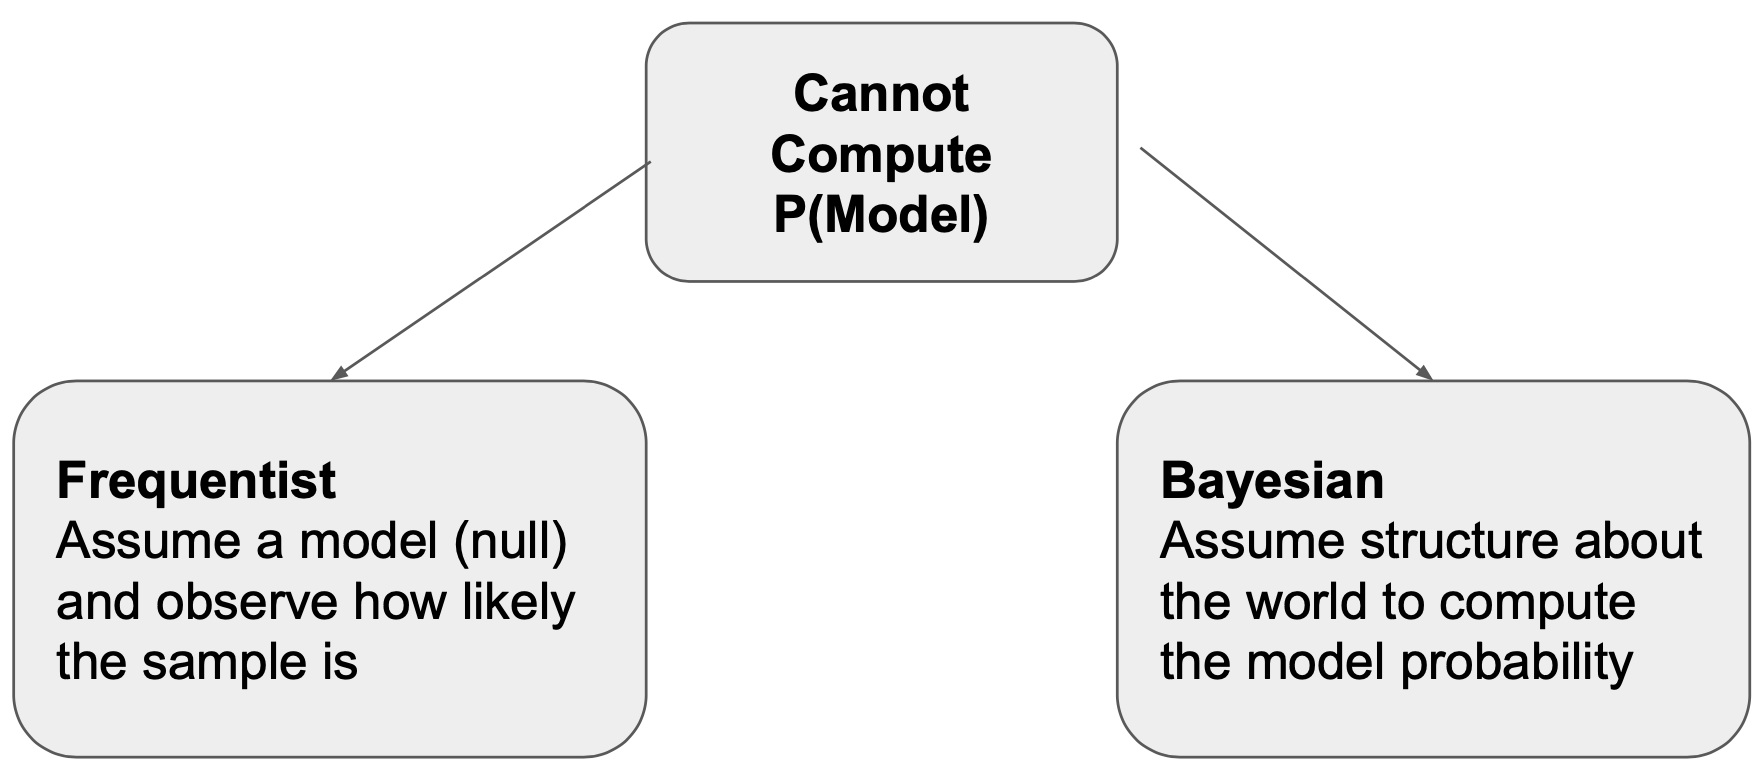
\includegraphics[width=.9\linewidth]{./figures/two_worlds}
\end{frame}

\section{The Frequentist Approach}

\begin{frame}
  \frametitle{The Birth of Modern Statistics}
    \begin{center}
        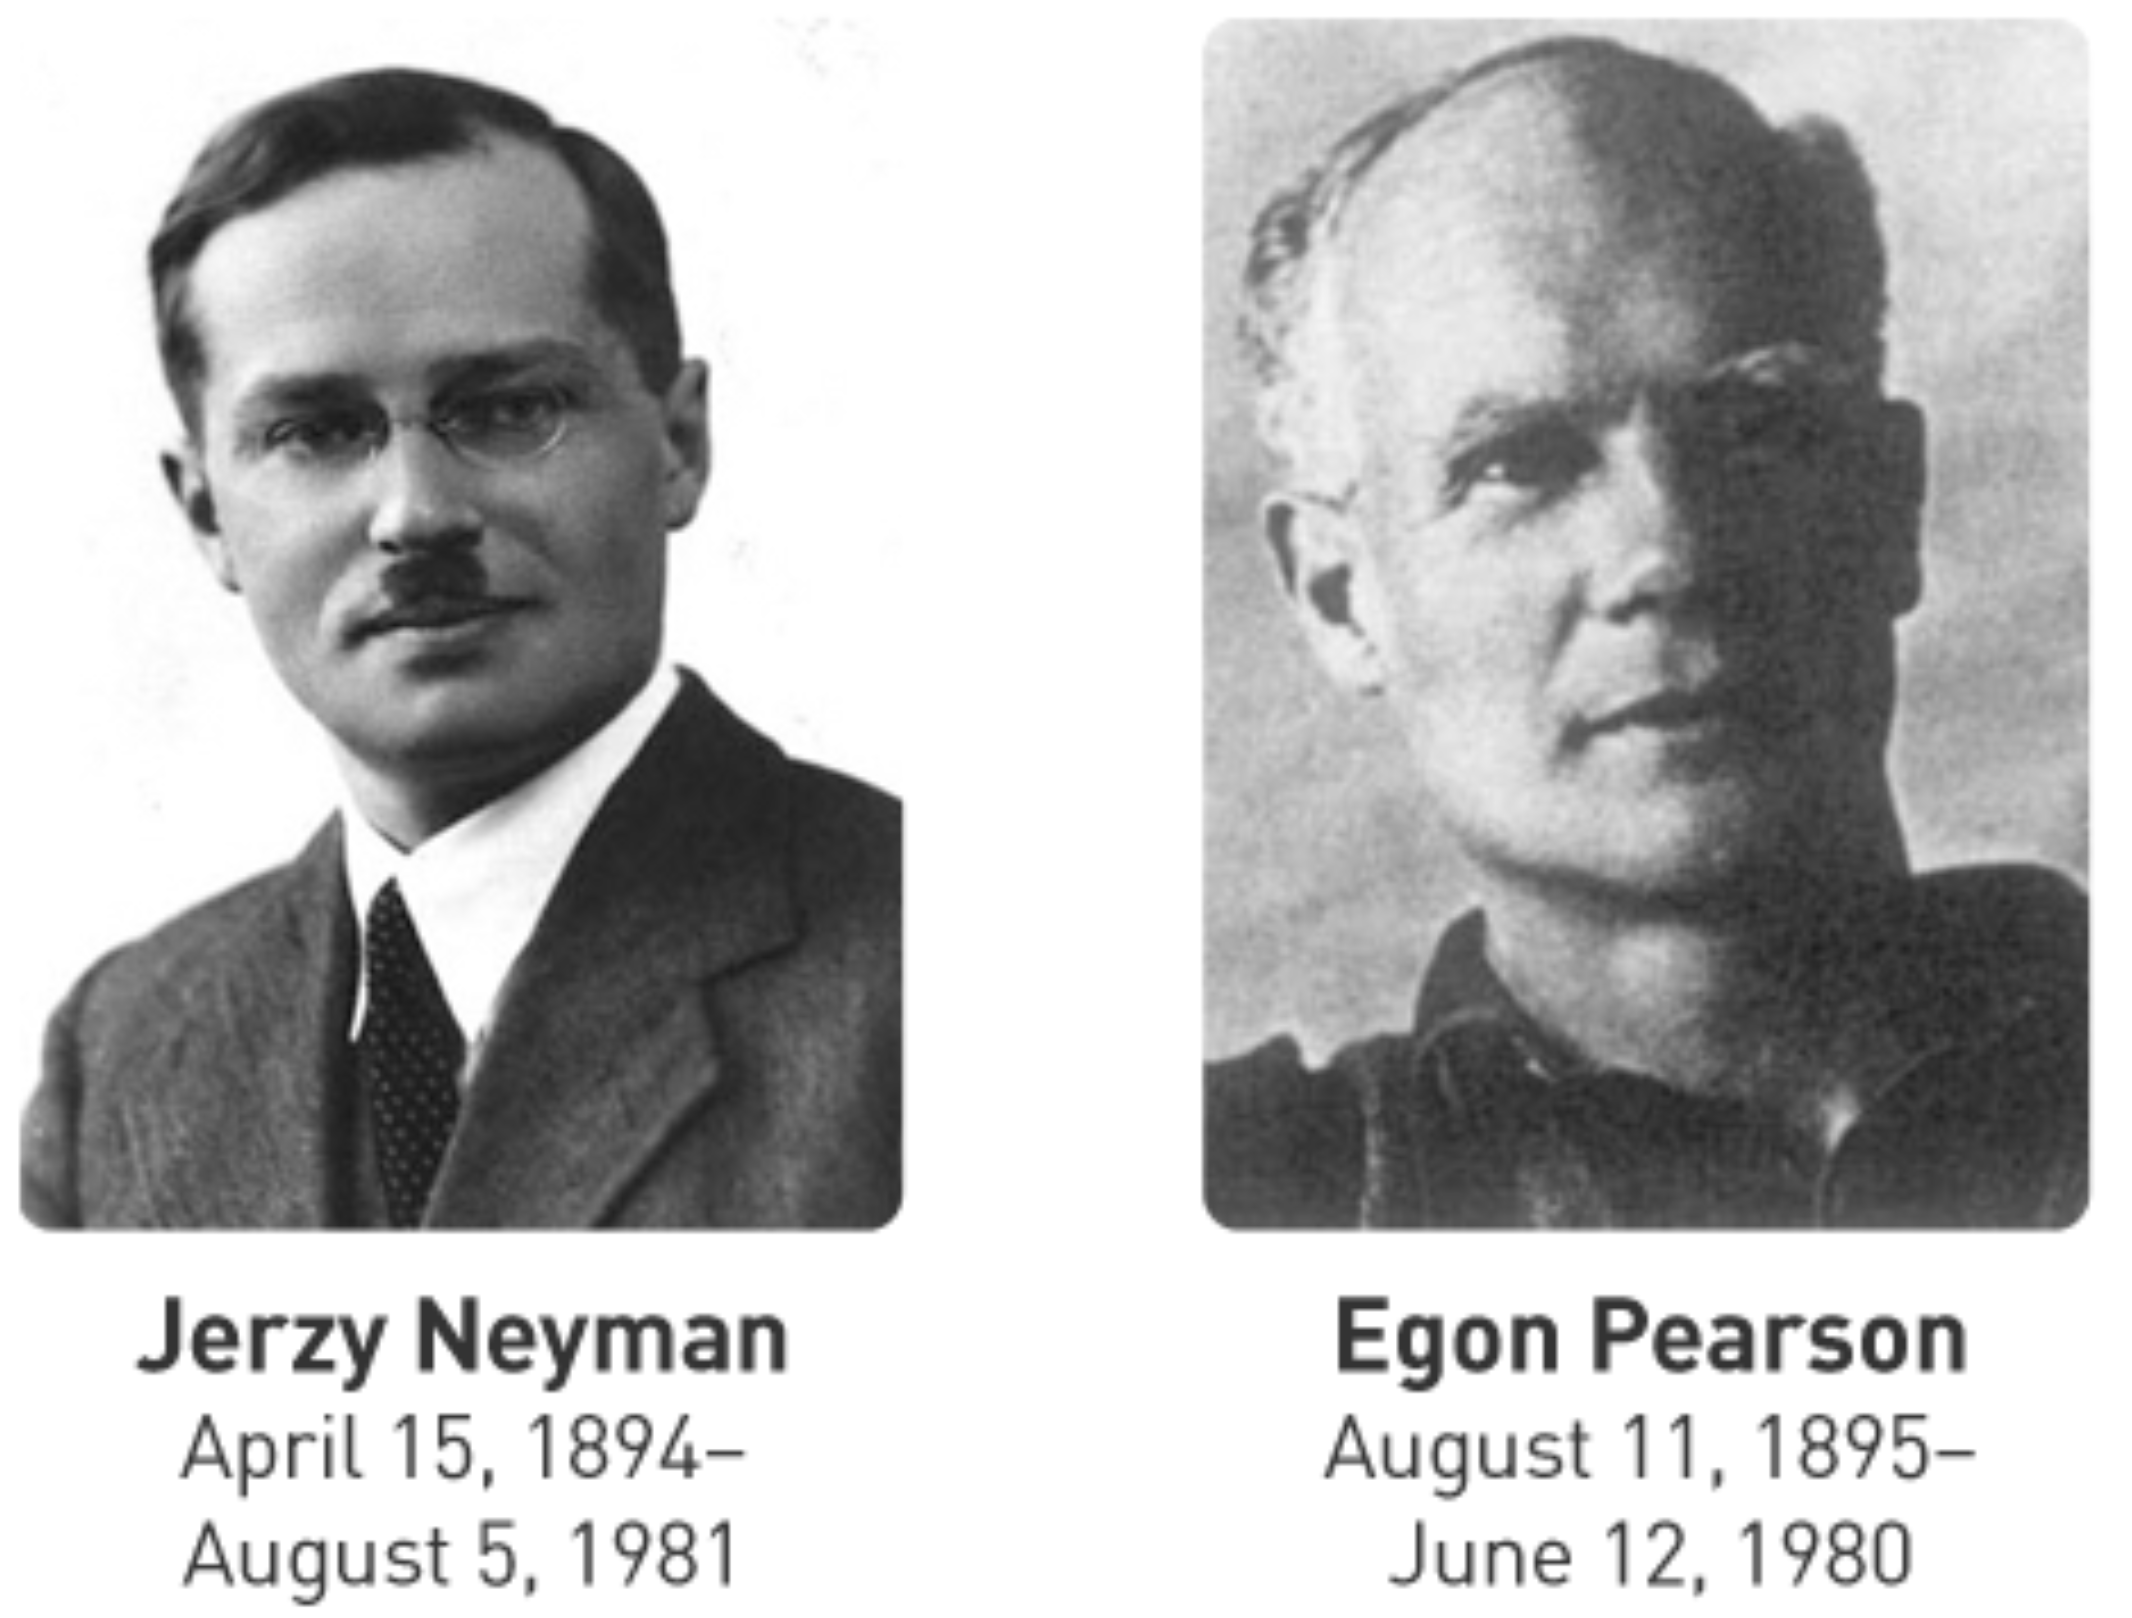
\includegraphics[width=0.4\textwidth]{figures/neyman_and_pearson.png}     
    \end{center}

  \begin{itemize}
      \item Before the 1930's, there were lots of statistical procedures but no coherent account of how to choose the right one
      \item Neyman and Pearson published articles that added a rigorous mathematical treatment, forming the basis of frequentist statistics
  \end{itemize}
\end{frame}

\begin{frame}
  \frametitle{The Central Dilemma}
  \begin{itemize}
      \item We observe data, $D$
      \item Given that this data occurs, we want the probability that our hypothesis $P(H|D)$ is \textbf{true}
  \end{itemize}
  
  To a strict frequentist:

  \begin{itemize}
      \item Not just impossible to compute
      \item Does not even make sense to assign a probability to a hypothesis
  \end{itemize}
\end{frame}



\begin{frame}
  \frametitle{Objective Probability}
  A frequentist defines probability as a matter of long-run frequencies
  \begin{itemize}
    \item We need to specify a collective of elements
    \begin{itemize}
        \item Eg. throws of a dice
        \item \textbf{Collective:} a frame of observations that can happen over and over
    \end{itemize}
    \item As number of observations approaches infinity, proportion of throws of the die that show a 3 is 1/6
    \item The probability is the long-run frequency of the event relative to all observations (or of 3's relative to all throws)
    \begin{itemize}
        \item Called \textbf{objective probability}
    \end{itemize}
\end{itemize}
\end{frame}


\begin{frame}
  \frametitle{Objective Probability and Hypothesis}
  \begin{itemize}
    \item If you view probability as objective, you cannot talk about the probability of a hypothesis
    \item it is just true or false
    \item \textbf{Subjective Probability:} The probability of a hypothesis
    \begin{itemize}
        \item Allows for disagreement about what it is
        \item Reflects our lack of information
    \end{itemize}
  \end{itemize}

  \textbf{So, what probabilities can we study?}

  \begin{itemize}
    \item We need a long-run collective
  \end{itemize}
\end{frame}

\begin{frame}
  \frametitle{$PR(D|H)$}
  \begin{itemize}
    \item $H$ = hypothesis
    \item $D$ = data
  \end{itemize}

  Assume H is true and call it the null hypothesis

  \begin{itemize}
    \item Has to be quite specific (the only extra assumption we're making)
    \item Is the basis for predictions we need to make about what data should come out of the experiment
    \item Governs how the experiment behaves as we run it over and over
  \end{itemize}
\end{frame}

\begin{frame}
  \frametitle{$PR(D|H)$ (cont.)}
  Now we have a meaningful collective
  \begin{itemize}
    \item Can look at the relative frequencies of different outcomes
    \item Can specifically look at the number of hypothetical experiments in which we would get data at least as extreme as D
    \begin{itemize}
        \item Captured by $p$-value
        \item \textbf{\textit{p}-value:} The probability of getting data as extreme as our observations, assuming the null hypothesis is true
    \end{itemize}
  \end{itemize}
\end{frame}

\section{Decision Rules}

\begin{frame}
  \frametitle{Hypothesis Test Example}

  \begin{exampleblock}{Mad data science}
    Suppose that your lab has synthesized a new compound, 
    \textit{Vitamin W}.

    Let random variable $B$ represent the change in blood pressure that results from taking
    \textit{Vitamin W}.
    
    Let $\mu = \E[B]$.

    You need to make a decision, to invest resources in Vitamin W or not. 
  \end{exampleblock}
  
  \note[item]{Let's use a stylized example to motivate the hypothesis testing framework.}
   
 \end{frame}

\begin{frame}
  \frametitle{Two Possible States of the World}
  \textbf{Goal:} Begin with a reasonable default supposition; leave
  this supposition behind if data provides compelling evidence
  \begin{columns}[t]
    \column{.5\linewidth}
    \textbf{Null hypothesis}
    \begin{itemize}
    \item Default assumption, status quo, statement that data might overturn
    \item  $H_\varnothing: \text{Usually } \mu=0$
    \item No effect
    \end{itemize}
    \column{.5\linewidth}
    \textbf{Alternative hypothesis}
    \begin{itemize}
    \item Idea or alternative to status quo
    \item $H_a:$ Usually  $\mu \neq 0$
    \item Some effect exists
    \end{itemize}
  \end{columns}
  
  With compelling evidence, we leave the specific null hypothesis
  ($H_{\varnothing}$) for the alternative ($H_{a}$)
\end{frame}

\begin{frame}
\frametitle{A Hypothesis Test}

A \textit{hypothesis test} is a procedure.

\begin{center}
  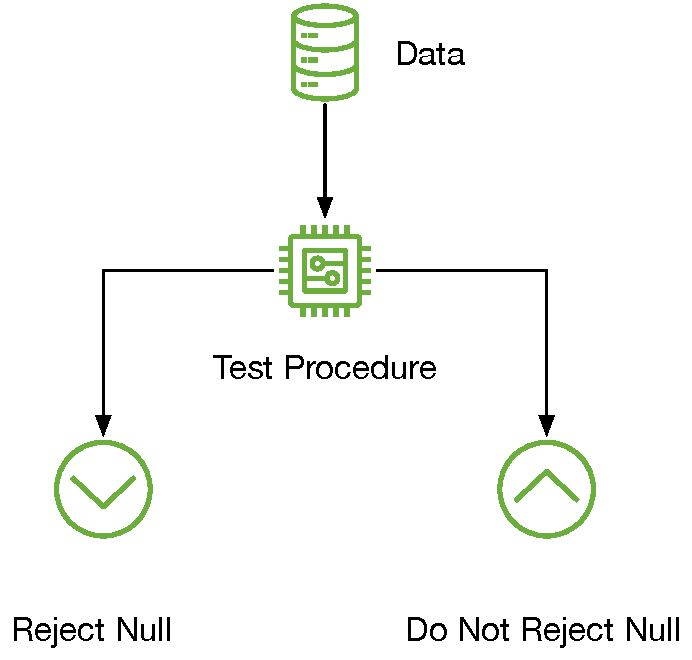
\includegraphics[width=.65\textwidth]{figures/test_procedure}
\end{center}
\note[item]{This is very strict: you might want your hypothesis test
  to do more, to give you fine-grained information about the world.
  but statistics doesn't work like that.  All we can do, is set up a
  specific null hypothesis and make this binary decision: reject or
  not reject.} 
\end{frame}


\begin{frame}
  \frametitle{False Positive and False Negative Errors}
  \begin{center}
    \small
    \begin{tabular}{p{3cm}| p{3cm}| p{3cm}}
      & \multicolumn{2}{c}{\textbf{True state of the world}}  \\ 
      & \textit{The null is true} & \textit{The null is false} \\
      \hline \hline 
      \textit{Reject the null} & False Positive & \\
      & (Type I Error) & \\
      \hline 
      \textit{Do not reject the } & & False Negative\\
      \textit{null}&& (Type II Error)
    \end{tabular}
  \end{center}
\end{frame}

\begin{frame}
  \frametitle{False Positive and False Negative Errors (cont.)} 
  \textbf{False Positive Errors}
  \begin{itemize}
    \item Typically the most destructive
    \note[item]{Why?  Because we don't want to abandon our existing
      beliefs about the world too quickly - our existing beliefs are
      our beliefs for a reason.}
    \note[item]{The world has all these researchers testing different
      medications, we don't want to be flooded with treatments that
      don't actually work.}
    \note[item]{Once a single study finds a link between red wine and
      heart disease, it gets out into the papers, people start
      believing it, and there's no way to undo that. }
  \item Error rate, denoted $\alpha$, is the probability of rejecting
    the null hypothesis when we should not; $P(\text{Reject } H_\varnothing |
    H_\varnothing)$
  \item Starting with Ronald Fisher: set $\alpha = 0.05$
  \end{itemize} 
  
  A hypothesis test is a procedure for rejecting or not rejecting a
  null, such that the false positive error rate is controlled ($\alpha = 0.05$).
\end{frame}


\begin{frame}
  \frametitle{Breaking Down a Test Procedure}
  
  \textbf{A test statistic}
  \begin{itemize}
  \item A function of our sample
  \item Measures deviations from the null hypothesis
  \item Distribution must be completely determined by the null
  \end{itemize}

  \textbf{A rejection region}
  \begin{itemize}
  \item  A set of values for which we will reject the null
  \item  Chosen to be contrary to the null
  \item Total probability must be $\alpha = 0.05$
  \end{itemize}
\end{frame}

\begin{frame}
  \frametitle{What a Hypothesis Test Doesn't Do}

  \textbf{A hypothesis test does not prove the null hypothesis.}
  
  \begin{itemize}
  \item We control Type 1 error rates
    \note[item]{Throughout, can we refer to these as false positives
      and false negatives? Or, at the very least, can we be really
      clear about defining once what we mean by type-one and type-two
      errors? This is a pet peeve of mine.} 
  \item We cannot control Type 2 error rates
  \item How can you be sure the real B is not 0.01?  Or 0.00001?
    \note[item]{I'm not sure what we mean with this last point?} 
  \end{itemize}
  
    \textbf{Never accept the null hypothesis.}
\begin{itemize}
\item The valid decisions are reject and fail to reject.
\end{itemize}

  
\end{frame}

\section{The One-Sample z-Test}

\begin{frame}[t]
  \begin{exampleblock}{Vitamin W Example} 
    Suppose $(B_1,..,B_{100})$ are i.i.d. random variables with mean $\mu = \E[B]$, representing changes in blood pressure.
    
    Assume $B \sim N(\mu, \sigma)$.  Assume we know $\sigma[B]=20$.
      \end{exampleblock}
      
      \note[item]{We want to know if Vitamin W has an effect.  so we write $H_0: \mu = 0$.}
      \note[item]{We need a statistic, and a rejection region}
      \note[item]{For our statistic, we usually want to find something that follows a famous distribution.}
      \note[item]{Can use the standardized mean. $z = \frac{\bar{B}}{2} \sim N(0,1)$}
\note[item]{For our rejection region , we need to choose a subset of the real numbers.  I'll show you the most common choice, above 1.96 and below -1.96.}
\note[item]{Why these numbers?  If you integrate, you get a probability of 0.05.}
\note[item]{Ex: $\overline{B} = -5$. then $z = 2.5$ REJECT}
\vspace{.5cm}
   \begin{flushright} 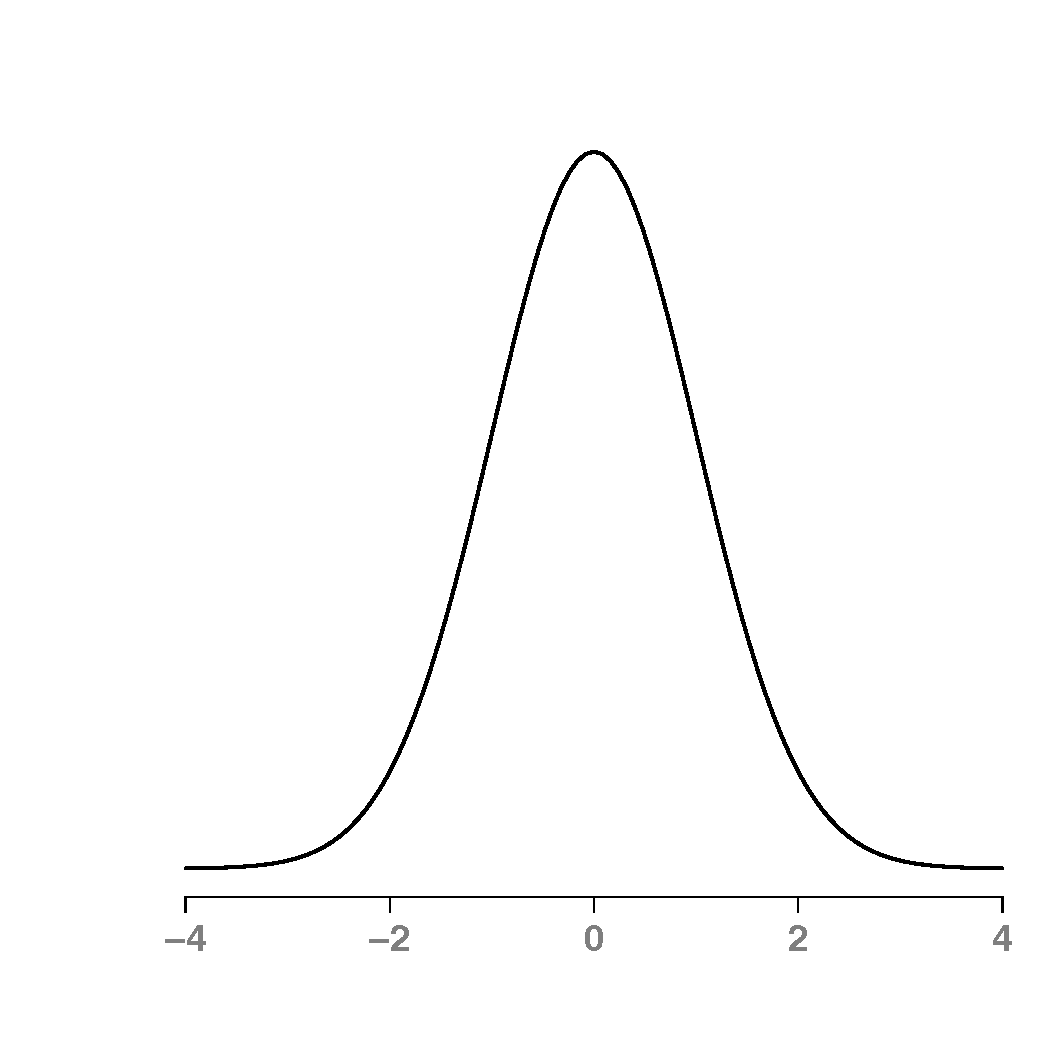
\includegraphics[height=.5\textheight, width = .5\textwidth]{figures/normal.pdf}
\end{flushright}
\end{frame}




% \section{Decision Rules Concept Check}

% \begin{frame}
%   \frametitle{Decision Rules Concept Check}

%   \begin{exampleblock}{A magician}
    
%     A magician gives you a coin. You want to run a test to see if it
%     is a fair coin.
% 
%     Your null hypothesis is that the coin is fair, and so has a
%     probability of heads that is $1/2$.
% 
%     You decide that you are going to flip the coin five times and declare
%     the coin to be unfair if the total number of heads is either zero
%     or five. \textbf{What is the Type 1 (false positive) error rate
%     for your procedure?}
% 
%     \begin{itemize}
%     \item $2 / 32$ 
%     \item $1 / 10$
%     \item $1 / 2$
%     \item $30 / 32$
%     \end{itemize}
%    
%   \end{exampleblock}
% \end{frame}

% \begin{frame}
%   \frametitle{Decision Rules Concept Check (cont.)}

%   \begin{exampleblock}{A magician}
%     \begin{itemize}
%     \item $\mathbf{2 / 32}$ -- There are 32 ways that the coins
%       \textit{might} fall, each of them equally probable. If the coin
%       \textit{were} fair in this is your rejection criteria, then you
%       will be wrong 2 of the 32 times.
%       \item $1 / 10$
%       \item $1 / 2$
%       \item $30 / 32$
%         
%       \end{itemize} 
%     \end{exampleblock}
% 
% \end{frame} 

\section{One- and Two-Tailed Tests}

\begin{frame}
  \frametitle{The Two-Tailed z-Test}

\begin{center} 
    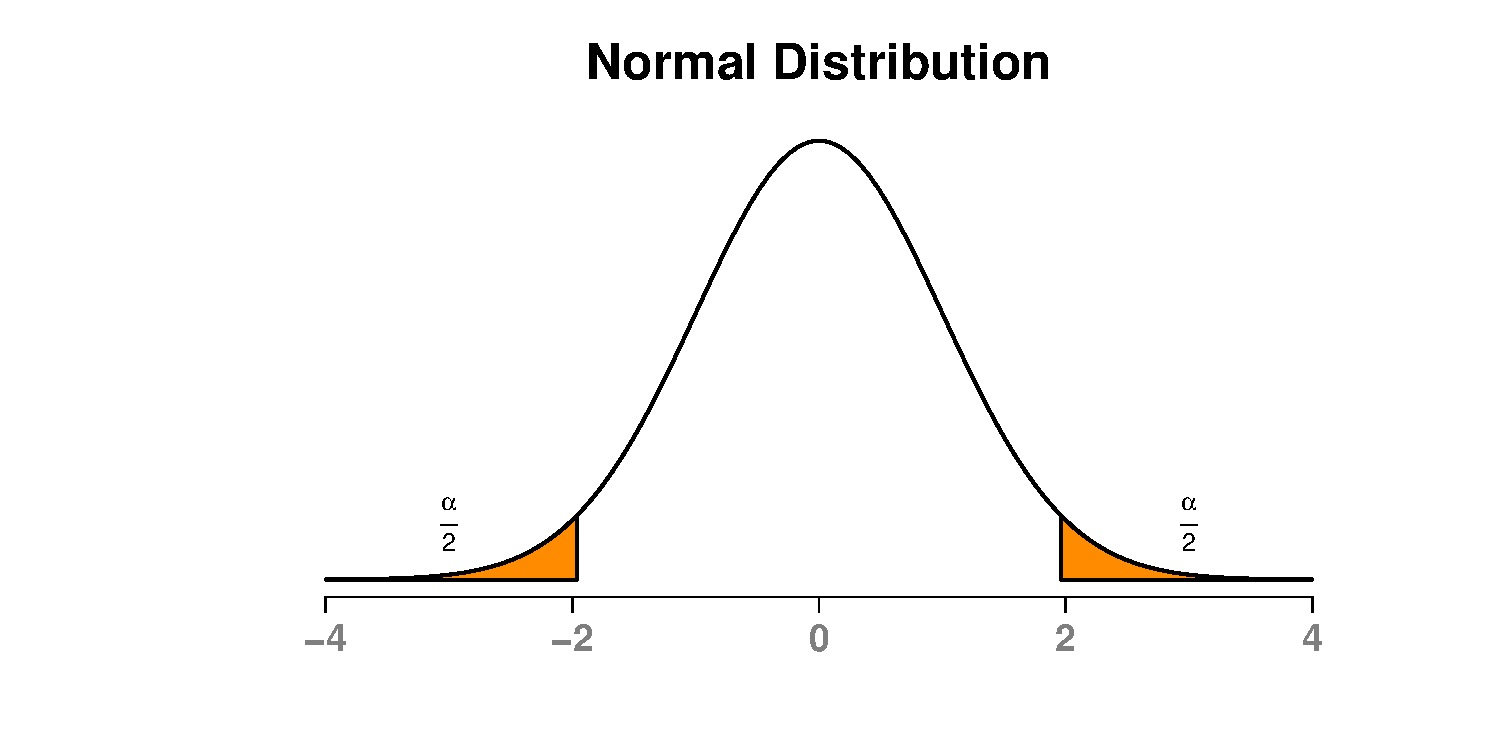
\includegraphics[width=\linewidth]{figures/normal_with_two_tails}
  \end{center}
  \begin{itemize}
  \item \textbf{Null hypothesis}: $\mu = 0$
  \item \textbf{Alternative hypothesis}: $\mu \neq 0$
  \end{itemize} 
\end{frame}

\begin{frame}
  \frametitle{The One-Tailed z-Test}
  \begin{center}
    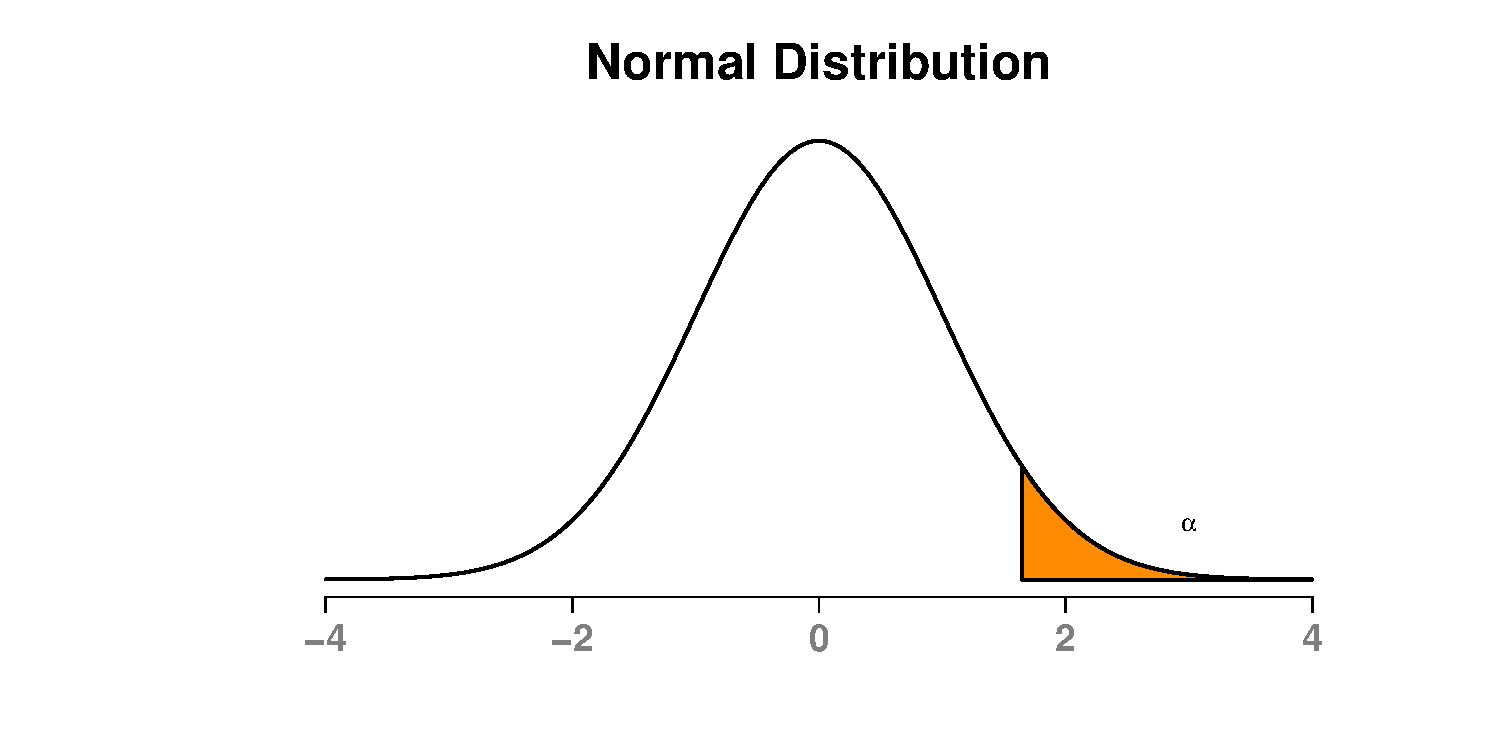
\includegraphics[width=\linewidth]{figures/normal_with_one_tail}
  \end{center}
  \begin{itemize}
  \item \textbf{Null hypothesis}: $\mu = 0$
  \item \textbf{Alternative hypothesis 1}: $\mu > 0$
  \item \textbf{Alternative hypothesis 2}: $\mu < 0$ 
  \end{itemize}
\end{frame}

\begin{frame}
  \frametitle{Choosing One or Two Tails} 

  \note[item]{One-tailed and two-tailed tests ask different questions, and are
  \textit{not} interchangeable.}
  \note[item]{It is kind of like being ID when you're buy a beer --
    they're not asking, ``Is this person different from 21?'' They're
    asking, ``Is this person older than 21?''}

  \begin{center}
    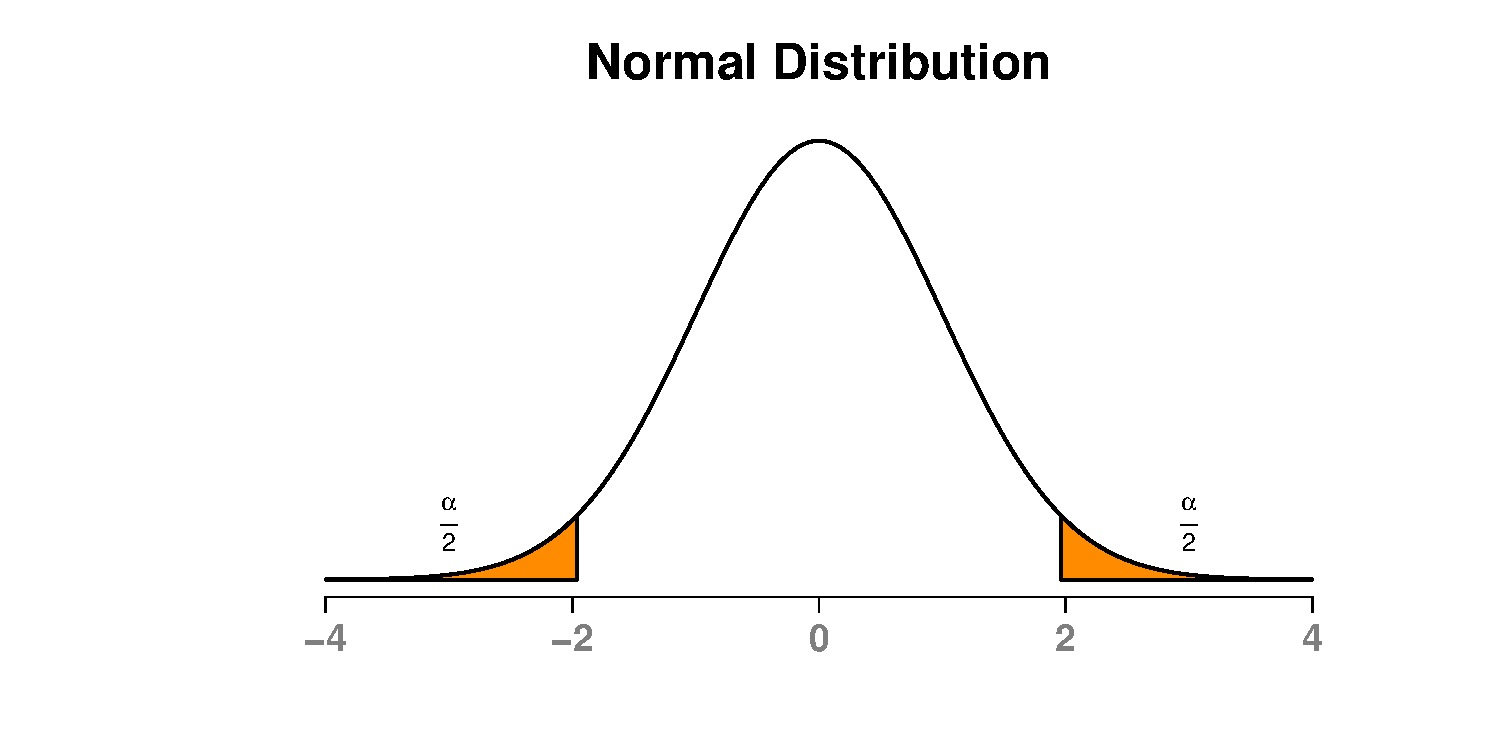
\includegraphics[width=0.6\textwidth]{figures/normal_with_two_tails} \\
    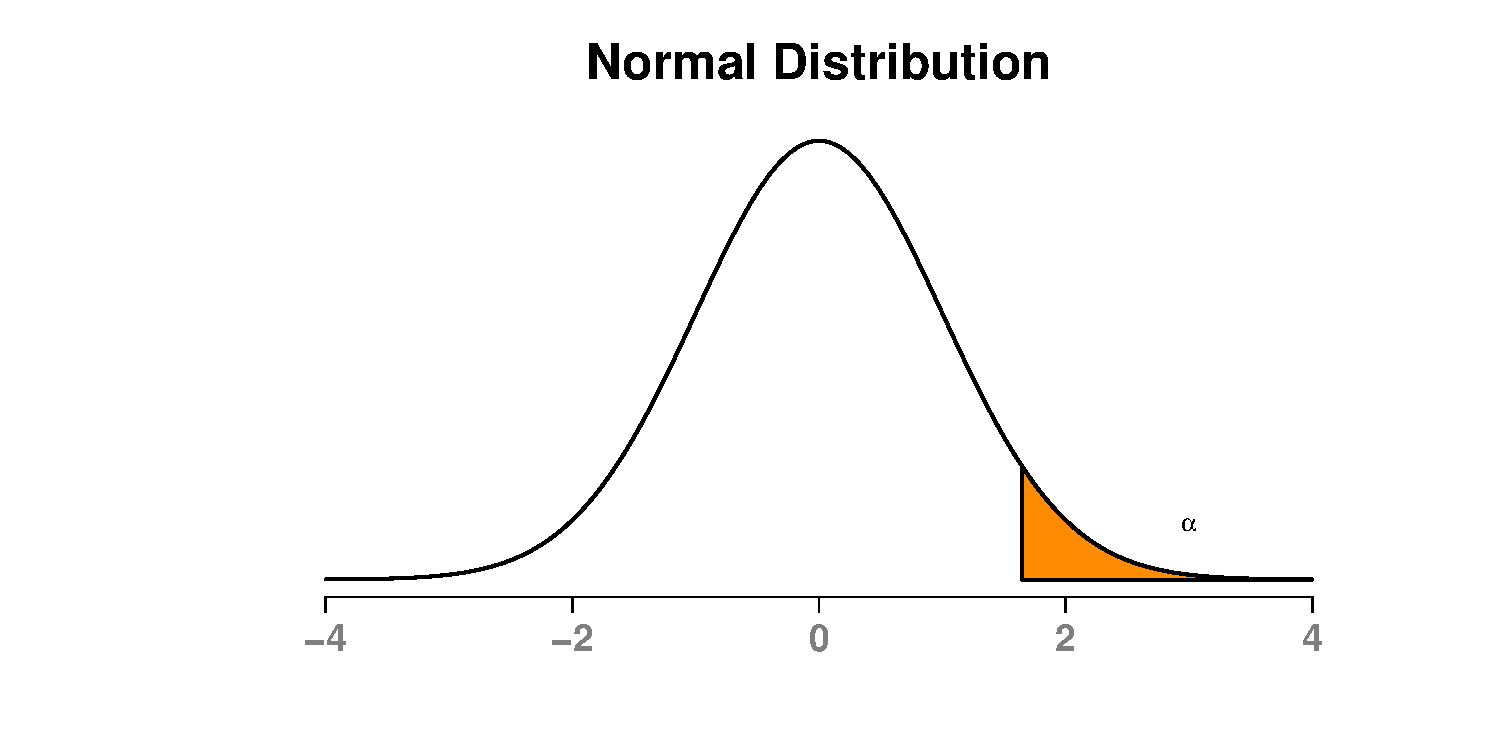
\includegraphics[width=0.6\textwidth]{figures/normal_with_one_tail}
  \end{center}

Switching your test after you see the statistic is cheating.
\end{frame}


\begin{frame}
\frametitle{One-Tailed Test: Things to Consider}

Before using a one-tailed test, ask yourself these questions:
\note[item]{``Do you feel lucky, punk? Well do ya?''}

\begin{enumerate}
\item Will the audience believe that I started with one tail before I saw the data?
\item Will the audience share my opinion of which tail is interesting?
\item Am I really 100\% committed to only this tail?
  \begin{itemize}
  \item What if the effect turns out to be huge, but in the other direction?  
  \item Would I be willing to call that a negative result?
  \item Can I convince my audience I have this much commitment?
  \end{itemize}
\end{enumerate}
\end{frame}

\section{T-Test Assumptions}

\begin{frame}
  \frametitle{T-Test Assumptions, Part I}

  \begin{block}{Assumptions of t-test}
    The textbook assumptions
    
    \begin{itemize}
    \item $X$ is a metric variable.
    \item $\{X_1,X_2,...,X_n\}$ is a random sample.
    \item $X$ has a normal distribution.
    \end{itemize}
    \end{block} 
    
    Variables are almost never normal.
    \note[item]{And so, these assumptions are nearly never met in practice}
\end{frame}

\begin{frame}
  \frametitle{T-Test Assumptions, Part II}
  
  But, in the large sample case, this is more plausible.

  \begin{block}{Large sample t-test assumptions} 
    \textbf{If}: 
    \begin{itemize}
    \item $X$ is a metric variable
    \item $\{X_1,X_2,...,X_n\}$ is a random sample
    \item $n$ is large enough that the CLT implies a normal distribution of mean
    \end{itemize}
    \textbf{Then}: The t-test is asymptotically valid
    \end{block} 
\end{frame}

\begin{frame}
  \frametitle{T-Test Assumptions, Part III}
  
\end{frame} 

\begin{frame}
  \frametitle{T-Test Assumptions, Part IV}
  
  The t-test is considered "reasonably robust," even when $n<30$, as
  long as deviations from normality are moderate.

  However, watch out for strong skewness, especially when $n<30$.

  \note[item]{DAH: We've got to give students more to work with than
    this; I think that this might end up being unsatisfying for many
    folks.} 
\end{frame}

\foreach \n in {1,...,36} {
  \begin{frame}{Gamma With Increasing Skew}
    Twenty draws from gamma distributions
    \begin{center}
      \includegraphics[width=\linewidth]{figures/gamma_skew_plots/gamma_skew_\n.pdf}
    \end{center}
  \end{frame}
}

\begin{frame}
  \frametitle{T-Test Assumptions}

  More practical guidance:
  
  \begin{itemize}
  \item $X$ is a metric variable.
  \item $\{X_1,X_2,...,X_n\}$ is a random sample.
  \item The distribution is not too non-normal, considering $n$.
  \end{itemize}
  
  When the t-test is not valid, consider using a non-parametric test instead.
\end{frame}

\section{Introduction to P-Values}

\begin{frame}
  \frametitle{Introducing P-Values}

  \begin{quote} The p-value is the probability, calculated assuming
    that the null hypothesis is true, of obtaining a value of the test
    statistic at least as contradictory to $H_0$ as the value
    calculated from the available sample.
  \end{quote}

\begin{flushright}
  \textit{ Jay L. Devore (2015)}
\end{flushright}

\note[item]{Let's note 2 things right away: just like in hypothesis
  testing.}  \note[item]{We're going to assume the null is true.}
\note[item]{We're measuring the probability of data - We may be
  interested in the probability that the null is correct - but
  statistics doesn't let us calculate that.}
\end{frame}

\begin{frame}
  \frametitle{Z-Distribution}
  
\end{frame}
  
\begin{frame}
  \frametitle{The P-Value for a Z-Test}
   
  \begin{exampleblock}{Vitamin W}
     
    You measure the effects of Vitamin W on blood pressure (measured
    in $mmHg$) for 100 patients and get $\bar{X} =3$.
     
    Assume $X \sim N(\mu,20)$.
     
    \begin{itemize}
    \item $H_0: \mu=0$
    \item $z = \frac{\bar{X} - \mu_0}{\sigma / \sqrt{n}} $
    \end{itemize}
  \end{exampleblock}
  \note[item]{ $= 3 - 0 / ( 20 / \sqrt{100} ) = 1.5$} \note[item]{$p =
    2*( 1- pnorm(1.5)) = 0.13$}
\end{frame}
 
\begin{frame}
  \frametitle{The P-Value and Decision Rules, Part I}

  Neyman-Pearson hypothesis testing: rules to make a decision and
  usually be right ($\alpha = 0.05$)

  \begin{exampleblock}{A classic z-test}
    \begin{itemize}
    \item z=1 $\rightarrow$ Do not reject null.
    \item z=2 $\rightarrow$ Reject null.
    \item z=10 $\rightarrow$ Reject null.
    \end{itemize}
  \end{exampleblock}

  \begin{itemize}
  \item Strict frequentist with a dichotomous decision rule: treat
    $z=2$ and $z=10$ identically.
  \item But is there value in knowing \textit{how contrary} the data
    is to the null?
  \end{itemize}
\end{frame}


\begin{frame}
  \frametitle{The P-Value and Decision Rules, Part II}
  \begin{align*}
    |z| & > \text{critical value} \Rightarrow \text{reject } H_{0} \\
    |z| & < \text{critical value} \Rightarrow \text{fail to reject } H_{0}
  \end{align*}

  \begin{center}
    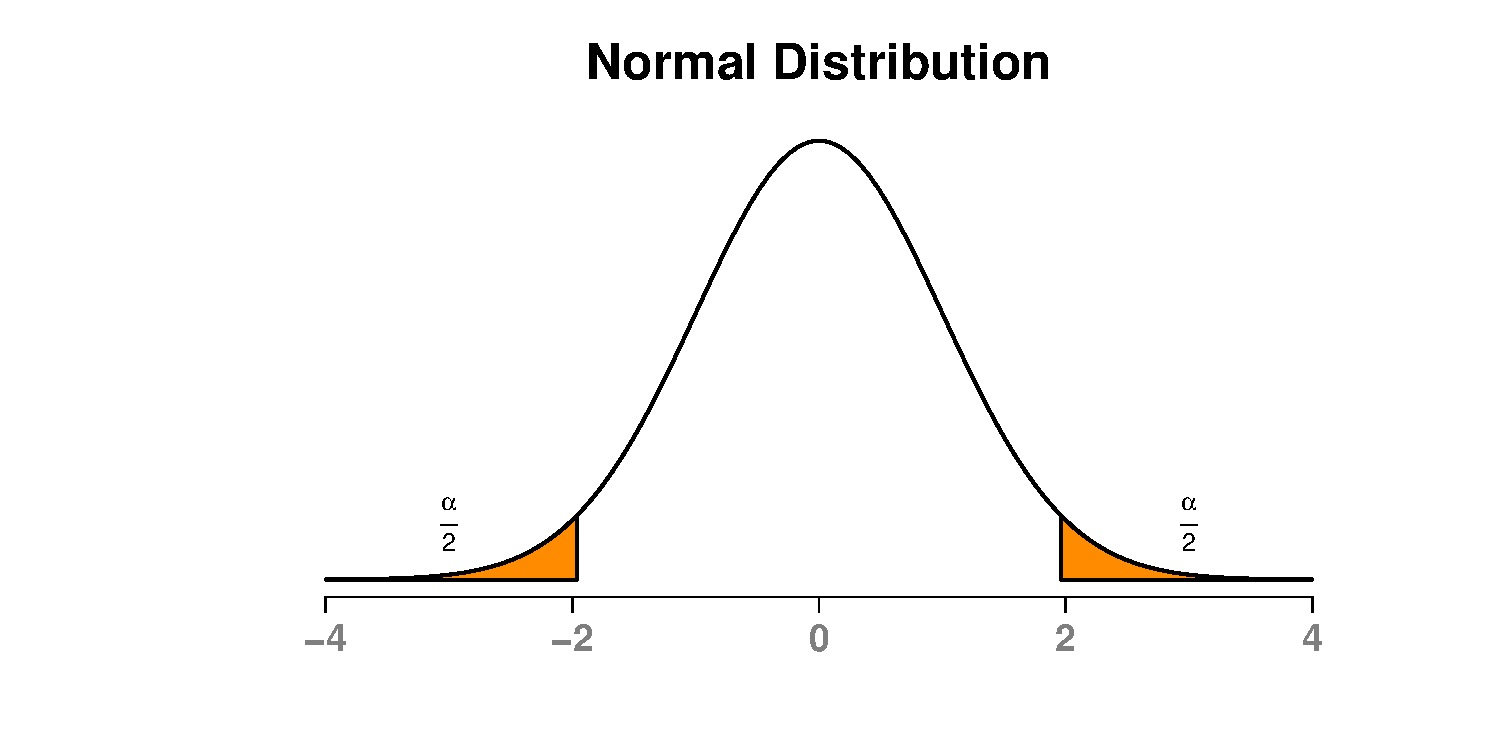
\includegraphics[width=\textwidth]{figures/normal_with_two_tails}
  \end{center}
\end{frame}

\begin{frame}
  \frametitle{The P-Value and Decision Rules, Part III}
  \begin{align*}
    |z| & > \text{critical value} \Rightarrow \text{reject } H_{0} \\
    |z| & < \text{critical value} \Rightarrow \text{fail to reject } H_{0}
  \end{align*}

  \begin{center}
    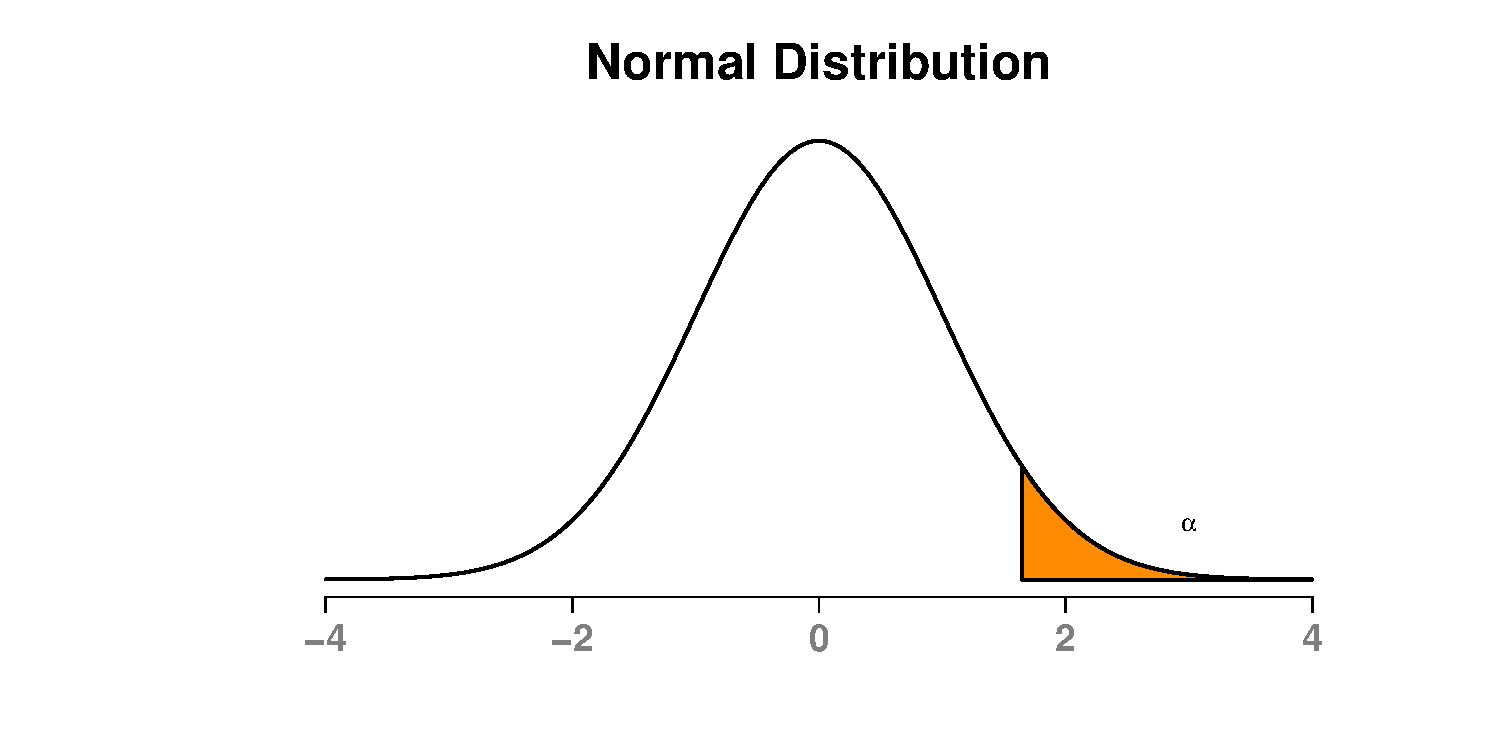
\includegraphics[width=\textwidth]{figures/normal_with_one_tail}
  \end{center}
\end{frame}

\begin{frame}
  \frametitle{An Equivalent Decision Procedure}
  
  Compute p-value.
  \begin{itemize}
  \item If $p<.05 \Rightarrow \text{reject } H_0$
  \item If $p\geq.05 \Rightarrow \text{do not reject } H_0$
  \end{itemize}
  But, can you justify making such a bright-line statement after
  reducing information so much?
  \begin{enumerate}
  \item Concept
  \item Measurement
  \item Statistic
  \item Assumptions about distribution
  \item \textbf{p-value}
  \item Reject/fail to reject
  \end{enumerate}
\end{frame}

\section{t-Test and p-Values} 

\begin{frame}
  \frametitle{P-Value Convention}
  
  \begin{center}
    \begin{tabular}{ c | c | c }
      p-value range & Convention  & Symbol \\
      \hline
      $p>0.10$ & Non-significant & \\
      \textcolor{textgray}{  $0.10 > p > 0.05$}  & \textcolor{textgray}{ Marginally-significant  } & . \\
      \hline
      $p<0.05$ & Significant & * \\
      $p<0.01$ & Highly significant & ** \\ 
      $p<0.001$ & Very highly significant & *** \\
    \end{tabular}
  \end{center}
\end{frame}
  
\begin{frame}
  \frametitle{Reporting Test Results}
  \begin{itemize}
  \item A t-test for the effect of Vitamin W on blood pressure was
    highly significant ($t=3.1$, $p=.008$).
  \item We found evidence that Vitamin W decreases blood pressure
    ($t=2.3$, $p=.04$).
  \item The effect of Vitamin X on blood pressure was not
    statistically significant ($t=1.2$, $p=.23$).
  \end{itemize}
  \vspace{.5cm}
  \begin{center}
    \begin{tabular}{ c | c }
      Vitamin W & Vitamin X \\
      \hline
      2.2 ** & 1.2 \\
      (0.6) & (0.8) \\
    \end{tabular} \\
  \end{center}

  This is half the story; next, you'll need to describe practical
  significance.

\end{frame}

\begin{frame}[t]
  \frametitle{Variable Importance and P-Values}
  Does a small p-value mean that a variable is ``important''?
  \begin{itemize}
  \item Statistical significance
  \item Practical significance
  \end{itemize} 
\end{frame} 

\begin{frame}
  \frametitle{A Warning}
  
  A very common mistake is to assume a p-value is the chance the null
  hypothesis is true.
  
  Frequentist statistics cannot tell you the probability of a
  hypothesis!

\end{frame}

\begin{frame}
  \frametitle{A Warning (cont.)}
  \begin{exampleblock}{Example}
    I test whether Vitamin X decreases blood pressure: $p = 0.03$.
  
    However, you know that Vitamin X is secretly cornstarch because
    you created it yourself.
  
    My test will not convince you that there is a 97\% chance Vitamin
    X decreases blood pressure.
  \end{exampleblock}
\end{frame}

\section{Statistical Power}

\begin{frame}
  \frametitle{False Positive and False Negative Errors}
  \begin{tabular}{ r | c | c  }
    & The null is true & The null is false \\
    \hline
    Reject the null & False Positive (I) & \\
    Do not reject the null & & False Negative (II) \\
  \end{tabular}
  \vskip 1cm
  
  \begin{itemize}
  \item False Positive (I) errors are jumping without cause
  \item False Negative (II) errors are failing to jump when you
    should
    
    \begin{itemize}
    \item Failing to detect a real effect
    \item Missed opportunity to create a product, publish a paper, or advance knowledge
    \end{itemize}
  \end{itemize} 
\end{frame}


\begin{frame}
  \frametitle{Statistical Power, Part I}

  \begin{exampleblock}{Much Vitamin W}
    Consider a \textit{specific} alternate hypothesis: 
    
    \begin{itemize}
    \item $H_a: $ Vitamin W decreases blood pressure by 20 mmHg
    \end{itemize}
  \end{exampleblock} 
  % you might wonder how we come up with that - maybe we decide that 20 mmHg is the minimum effect that would let us go to market.

  \begin{itemize} 
  \item False Negative Error Rate: $\beta = P(\text{not rejecting }H_0 | H_a)$
  \item Statistical power: $1-\beta$
  \item Statistical power is the probability of supporting the
    alternate hypothesis, assuming it is true
  \end{itemize} 
\end{frame}
  

\begin{frame}
  \frametitle{Statistical Power, Part II}

\begin{center}
  \centering
  \note[]{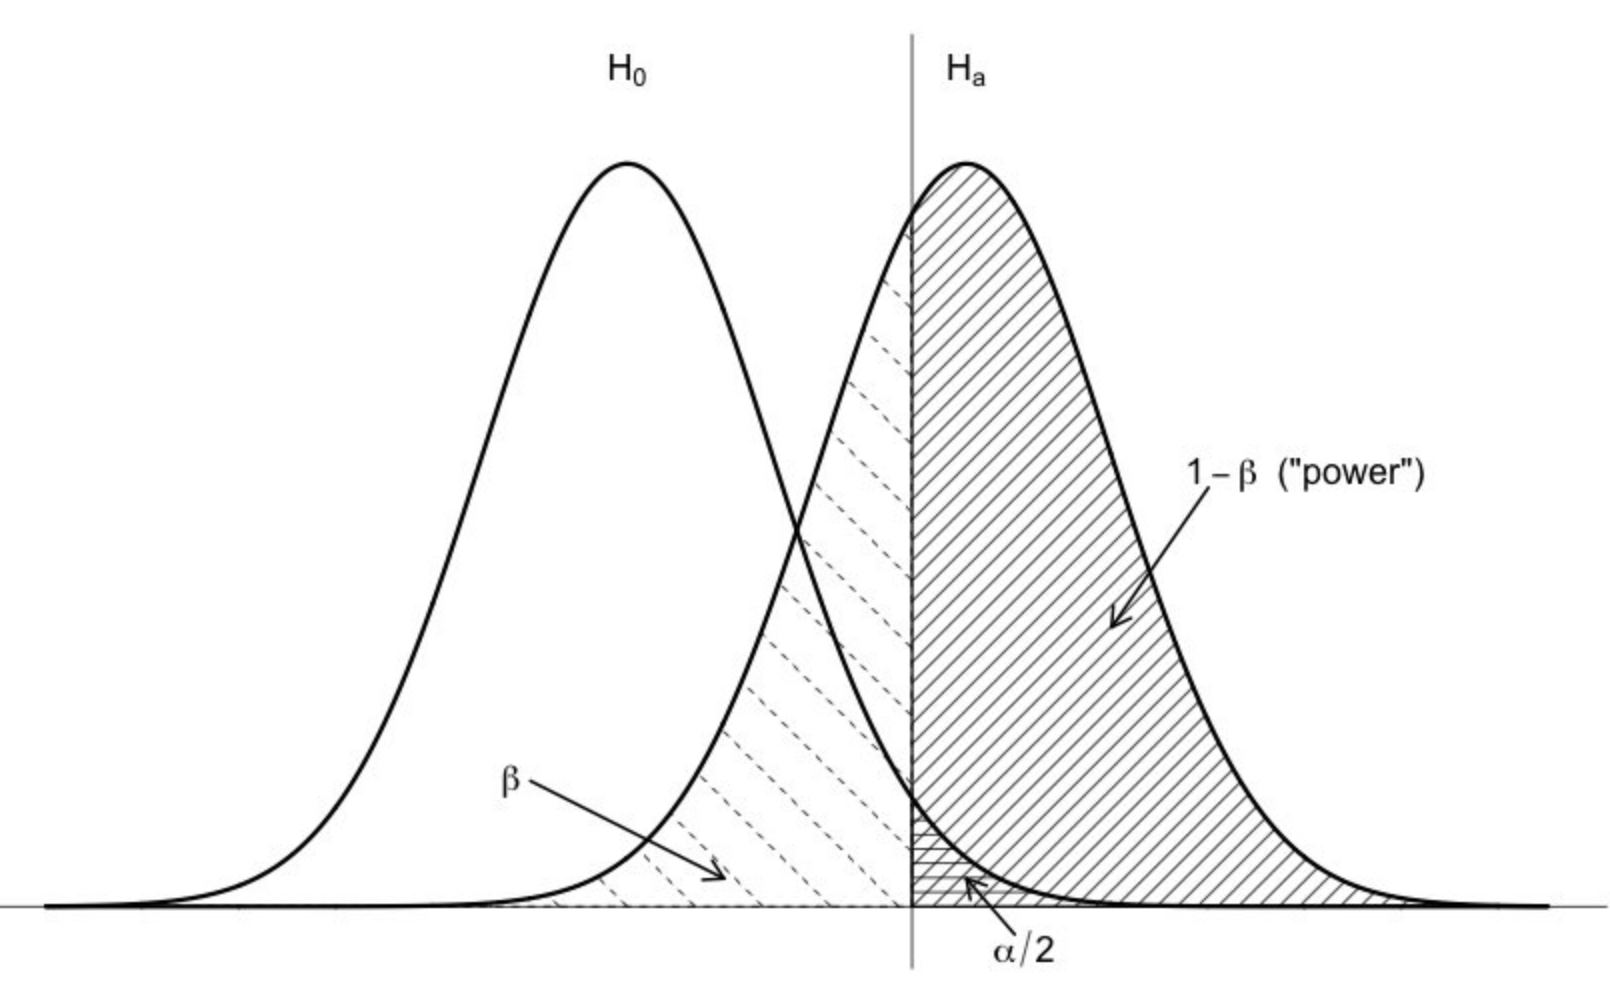
\includegraphics[width=\linewidth]{./figures/power}}
\end{center}
\end{frame}

\begin{frame}
  \frametitle{Statistical Power, Part II}
  
\end{frame} 

\begin{frame}
\frametitle{Statistical Power, Part III}

How to increase power
\begin{itemize}
\item Increase sample size.
\item Choose a powerful test (if you can justify its assumptions).
\end{itemize}

\end{frame}

\section{Practical Significance}

\begin{frame}
  \frametitle{Practical significance}
  \begin{block}{Statistical significance}
    \begin{itemize}
    \item How much does the data support the existence of an effect?
    \end{itemize}
  \end{block}
  \begin{block}{Practical significance}
    \begin{itemize}
    \item Is the size of this effect important?
    \item What is the magnitude of the effect?
    \item Should we care about this effect?
    \end{itemize}
  \end{block}
  \note[item]{In many cases, statistical significance is little more
    than a statement of how large a sample was used to test a
    question.}
\end{frame}
 
 \begin{frame}
   \frametitle{Example}
   \begin{exampleblock}{Productivity supplements}
     % Suppose that two studies examine how vitamin supplements affect
     % productivity.
     \vspace{1em}

     \begin{columns}[t]
       \column{0.42\textwidth}
       \textbf{Vitamin W}
       \begin{align*}
         n &= 30 \\ 
         \mu_{treat} &= 12.6 \\
         \mu_{control} & = 6.1 \\
         p &= 0.11
       \end{align*} 
        \textit{``The difference between groups was not
           statistically significant}, $(t=1.34, p=0.11$).''
       \column{0.42\textwidth}
       \textbf{Vitamin Q}
       \begin{align*}
         n &= 30,000 \\
         \mu_{treat} &= 6.25 \\
         \mu_{control} &= 6.21 \\
         p &= 0.0005
       \end{align*}
       \textit{``The difference between the two groups was highly
         significant}, $(t = 3.34, p<0.001)$.'' 
     \end{columns}
   \end{exampleblock}
 \end{frame}

 \begin{frame}
   \frametitle{Practical Significance: Context}
   \textbf{Primary goal}: Provide context for your audience to reason
   about results.
   \begin{itemize}
   \item Who is your audience? 
   \item What action might be taken based on these results?
   \item How does this result alter how you would run the business? 
   \item What is the cost-benefit for implementing a change based on
     this result? 
   \item How does this result ``stack up'' to other effects?
   \end{itemize}
   \note[item]{Understanding and communicating the business context is
     what separates good analysts from great data scientists.}
   \note[item]{One might be very certain of a very small increase in a
     desirable metric; one might be less certain of a very large
     increase in a desirable metric.} 
   \note[item]{In many places, every relationship examined is
     significant. But, what do they \textit{mean}?} 
   \note[item]{We should directly tie this in to the machine learning
     conversation they're going to have in 207 about feature
     importance.} 
 \end{frame}

 \begin{frame}
   \frametitle{Practical Significance: Model Explainability}
   \begin{itemize}
   \item Some tasks require \textit{explainable} models.
   \item Finance, healthcare, insurance, and other regulated industries
     stipulate specific model forms .
   \item Humans reason in linear hypotheses— higher-dimensional
     and conditional hypotheses are too much to keep in
     mind.
   \end{itemize}
 \end{frame}

\begin{frame}
  \frametitle{Practical Significance: Effect Sizes}
  \begin{block}{Effect sizes} 
    \begin{itemize}
    \item Single-number metrics that characterize the
      magnitude of an effect
    \item Population parameters that we estimate—\textit{do not vary
        based on sample size}
    \end{itemize}
  \end{block}
  \vspace{1em} 
  \begin{columns}[t]
    \column{0.49\linewidth}
    \textbf{Invalid effect size metrics}
    \begin{itemize}
    \item t-stat
    \item p-value 
    \end{itemize}
    \column{0.49\linewidth}
    \textbf{Valid effect size metrics} 
    \begin{itemize}
    \item Mean values 
    \item Difference in means between groups
    \end{itemize}
  \end{columns} 
% Headline Test: What single number can you put in a newspaper
% headline to get the importance across? 
% \begin{itemize}
% \item Ex: Vitamin W increases lifespan by 1.2 years.
% \end{itemize}
\note[item]{This headline test feels out of place relative to the
  other content on this section.}
\end{frame}

\begin{frame}
  \frametitle{Standard Effect Size Measures}
  Standardized effect sizes are designed to be flexible and apply in
  many scenarios:
  \begin{itemize}
  \item Cohen's $d$
  \item Correlation $\rho$
  \item Cramer's $V$
  \end{itemize}
  General metrics ignore the specific context around your research or
  business question.
  \note[item]{These provide general guidance about whether an effect
    is small, medium, or large.}  
  \end{frame}


\begin{frame}
  \frametitle{Cohen's d}
    Sometimes, a mean (or difference in means) is hard to assess because
  the units are unfamiliar.
  \begin{itemize}
  \item \textbf{Example}: The effect of angled bristles on tooth decay
    is 5 millicaviparsecs per
    brushstroke %% TO THE REVIEWERS: Yes, we know this isn't a word
  \end{itemize}
  \begin{block}{Cohen's d} 
    Compare effect size relative to the underlying natural variation
    in the outcome.
    \[
      \text{Cohen's } d = \frac{\text{mean difference}}{\text{standard
          deviation}}
    \]
    \end{block} 
\end{frame}

\begin{frame}
  \frametitle{Cohen's d (cont.)}
  \begin{center}
  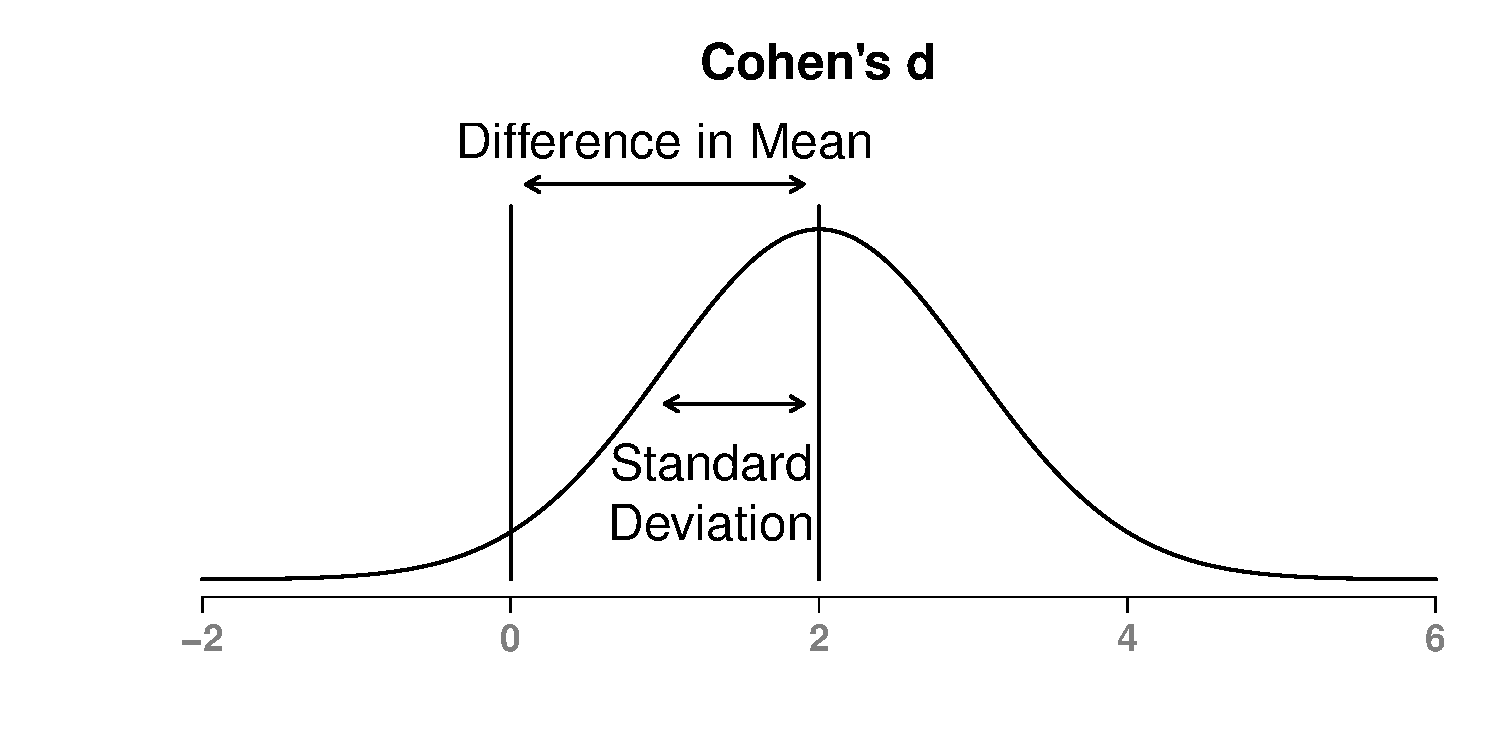
\includegraphics[width=\linewidth]{./figures/cohens_d.pdf}
  \end{center}
\end{frame} 

\begin{frame}
  \begin{block}{Rules of thumb (according to Cohen)}
    \begin{center}
      \begin{tabular}{rc}
        Small effect     & $d = 0.2$ \\ 
        Medium effect & $d = 0.5$ \\ 
        Large effect      & $d = 0.8$ \\
      \end{tabular}
    \end{center}
  \end{block} 
  \begin{itemize}
    \item Applicable across a huge number of contexts 
    \item Ignores any important differences between context 
    \item Saving dollars or saving lives are the same to Cohen's d
  \end{itemize} 
\end{frame}

\begin{frame}
  \frametitle{Takeaways}
  \begin{itemize}
  \item  After a statistical test, it's important to assess both
    statistical significance and practical significance.
  \item Standard effect size measures can help in a wide variety of situations.
  \item But don't get carried away and reach for them automatically.
  \item The main objective is to clearly explain how important the
    magnitude of the effect is.
  \end{itemize}
\end{frame}

%Section 6.28 Edits start here
\section{Guidelines For Statistical Reporting}

\begin{frame}
  \frametitle{Guidelines for Statistical Reporting}
  \begin{itemize}
    \item Communicating your results is a key part of statistical analysis
    \item In this class (and other classes in the program) we'll ask you to submit your analysis as a written report
    \item Next are some guidelines to keep in mind when writing a report
  \end{itemize}
 
  \textit{In this case, the guidelines are specific to exploratory analysis}
\end{frame}

\begin{frame}
  \frametitle{Guideline One}
    \begin{exampleblock}{A statistical analysis is a written argument}
      \begin{itemize}
        \item A good writing style is key
        \item This is technical writing: aim for clarity and exposition
        \item All rules of good writing apply
        \begin{itemize}
          \item Organize your argument clearly
          \item Guide reader through the evidence in the data
          \item Proofread
        \end{itemize}
      \end{itemize}
    \end{exampleblock}
\end{frame}



\begin{frame}
  \frametitle{Guideline Two}
\begin{exampleblock}{If you don't have something nice to say (about your output), don't display it at all}
  \begin{itemize}
      \item There should be no output dumps
      \item Every graph should be mentioned in your writing and should have some purpose
      \item Explain what the graphs and numbers mean
  \end{itemize}
\end{exampleblock}
\end{frame}


\begin{frame}
  \frametitle{Guideline Three}
\begin{exampleblock}{You should document decisions}
  \begin{itemize}
      \item If you decide that observations should be removed, state which ones
      \item If values are suspicious, but you leave them in, state that too
      \item If you transform a variable, for example, by taking the logarithm, state that
      \item Your justification can often be very brief (just a sentence), but make sure that the reader can follow your logic
  \end{itemize}
\end{exampleblock}
\end{frame}



\begin{frame}
  \frametitle{Guideline Four}
  \begin{exampleblock}{Identify features that should be reflected in statistical models}
    \begin{itemize}
      \item This will make more sense once you have experience building models
      \item Keep in mind the purpose of the analysis
      \item Eg. if you're interested in explaining the price of a house, look to see what kind of relationship that variable has with the explanatory variables
        \begin{itemize}
          \item Is it linear?
          \item Is it exponential?
          \item Are there values that don't seem to fit with the overall trend?
        \end{itemize}
    \end{itemize}
  \end{exampleblock}
\end{frame}


\begin{frame}
  \frametitle{Guideline Five}
  \begin{exampleblock}{Remember the difference between sample and population}
    \begin{itemize}
      \item At this point, we don't know how to model a population
      This means that you must confine your conclusions to the sample
      \begin{itemize}
          \item You can talk about sample means, sample covariances
      \end{itemize}
      \item You can't say anything about the population that generated your sample
    \end{itemize}
  \end{exampleblock}
\end{frame}



\begin{frame}
  \frametitle{Guideline Five (cont.)}
  \begin{exampleblock}{Remember the difference between sample and population}
    \begin{itemize}
      \item Be wary of technical words--in particular the word \textit{significant}
      \begin{itemize}
          \item People might casually say one value is significantly bigger than another
          \item But this has a technical meaning, and it implies that we've built a model and performed a statistical test
      \end{itemize}
    \end{itemize}
  \end{exampleblock}
\end{frame}

\begin{frame}
  \frametitle{Guideline Six}
  \begin{exampleblock}{Show us the code (a guideline for this class)}
    \begin{itemize}
      \item We really want to see the code that generates your output so we can follow your analysis in detail, step by step
      \begin{itemize}
          \item Typically, your software will have a setting to suppress the code when generating a pdf report, but don't do it
      \end{itemize}
      \item This is probably the biggest difference between writing analyses in school and in a professional context
    \end{itemize}
  \end{exampleblock}
\end{frame}

\begin{frame}
  \frametitle{Guideline Six (cont.)}
  \begin{exampleblock}{Show us the code (a guideline for this class)}
    \begin{itemize}
      \item In most situations, you have to think about different levels of detail for different audiences
      \begin{itemize}
        \item It's usually a good idea to provide an executive summary
        \item Not everyone can read 50 pages of output
        \item Often, you'll want to move details like your script to an appendix
      \end{itemize}
      \item In this class, however, we'd like to see your code in the body of your report so we can evaluate it effectively
    \end{itemize}
  \end{exampleblock}
\end{frame}

\end{document}
